 \subsection{Otros.}
    \subsubsection{Módulo de WebScrapping - Wicked Fox}
    \paragraph{Este módulo será el encargado de tomar información de plataformas que carecen de un servicio web definido, por ejemplo el Sistema Meteolorógico Nacional. Toda la información que exponen de forma diaria, semana, mensual y anual. Se encuentra bajo un formáto HTML que puede ser visualizado a través de algún navegador web al acceder a su sitio.}
    \paragraph{Problemas cómo los anteriores suelen ser comunes a nivel nacional (principalmente plataformas gubernamentales), para poder hacer uso de esos recursos es necesario generar un módulo que de forma programática pueda extraer limpiar, extraer y adecuar la información.}
    \paragraph{Al proceso antes descrito se le conoce cómo \emph{Web Scrapping}\cite{6}, que se define cómo la extracción de información de sitios web a través de medios programáticos o programas definidos.}
    \paragraph{Éste módulo se encuetra implementado bajo un script escrito en Javascript usando PhantomJs cómo medio lógico y programático para la implemtación del Scrapping.}
    \paragraph{ La definición básica de \textbf{\emph{Wicked Fox}} es tomar el recurso que brinda el SMN, extraer la información contenida en tablas y posteriormente mandar esta información al módulo \textbf{\emph{Smart Owl}} que se encargará de adecuar y después delegar el trabajo al módulo de registro \textbf{\emph{Hard Ant}} donde al final la información climatológica de cierta localidad será guardad en alguna de las bases de datos antes mencionadas.}
      \begin{landscape}
        \begin{figure}[b!]
        \centering
        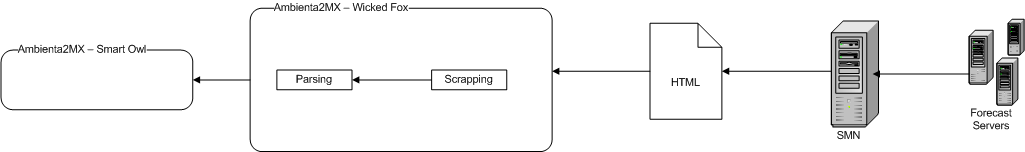
\includegraphics[width=19cm,height=4cm]{./images/DiagramaWickedFox.png}
        \caption{Diagrama General de Wicked Fox}
      \end{figure}
      \end{landscape}
    \paragraph{Éste módulo presenta una gran importancia debido a que actualmente se carece de un servicio a nivel nacional que brinde información meteorológica con cierta veracidad, si bien es cierto que otros sistemas extraen información de datos tomados por centrales mexicanas, el costo de éstos suele ser elevado.}
    \paragraph{La extracción de la información se ejecutará \emph{al vuelo}, es decir, éste proceso se ejecutará cada que se pidan datos con un margen no mayor a una hora de cierta localidad o ubicación del territorio nacional.}
    \paragraph{Para poder hacer uso de éste módulo es necesario brindar la información de la localidad via latitud/longitud o bien, a través de la localidad descrita, éstos datos serán proporcionados y resueltos por el módulo \textbf{\emph{Fast Eagle}} descrito anteriormente.}